%%%%%%%%%%%%%%%%%%%%%%%%%%%%%%%%%%%%%%%%%%%%%%%%%%%%%%%%%%%%%%%%%%%%%%%%
% Preamble
%%%%%%%%%%%%%%%%%%%%%%%%%%%%%%%%%%%%%%%%%%%%%%%%%%%%%%%%%%%%%%%%%%%%%%%%
\documentclass[11pt]{article}
%
% Packages and other includes
% Pagination
\usepackage[letterpaper, margin=1.25in]{geometry}
%
% Graphics, floats, tables
\usepackage{graphicx, color, float, array}
%
% Hyperlinks
\usepackage{hyperref}
%
% AMS packages for equations, math symbols
\usepackage{amsmath, amssymb, braket}
%
% Bibliography
\usepackage[style=numeric,sorting=none]{biblatex}
\addbibresource{references.bib}
%
% Revision (see Makefile)
\newcommand{\Revision}{977be36}

%
% Definitions and settings
% Paragraph indent and spacing
\setlength{\parskip}{0.4\baselineskip}
\setlength{\parindent}{0in}
%
% Math mode version of "r" column type (requires array package)
\newcolumntype{R}{>{$}r<{$}}
%
% Title, authors, date
\title{\textbf{Ensembles of Water-Halide Clusters}}
\author{Brian Nguyen and Luke Nambi Mohanam}
\date{Chem 150L Winter 2018 \\ \today, Revision \Revision}
%
%
%%%%%%%%%%%%%%%%%%%%%%%%%%%%%%%%%%%%%%%%%%%%%%%%%%%%%%%%%%%%%%%%%%%%%%%%
% Main document
%%%%%%%%%%%%%%%%%%%%%%%%%%%%%%%%%%%%%%%%%%%%%%%%%%%%%%%%%%%%%%%%%%%%%%%%
%
\begin{document}

\maketitle

\begin{abstract}
  Cluster models of water-halide solutions have been widely studied
  and have well-defined chemical composition. Often, certain ions
  have higher concentration
  closer to the surface at the air-water interface. In this report,
  a computational study of chloride-water clusters is investigated by
  determining local minima of a chloride cluster with 3 water,
  and comparing to experimental spectra.
  Two local minima structures were determined 
  with the difference of an
  additional hydrogen bond between water molecules. It is seen
  that the additional hydrogen bond led to a higher overall energy
  suggesting that there is some steric strain from forming the additional
  hydrogen bond.
\end{abstract}

\section{Introduction}

At the troposphere of the atmosophere, a complex combination of
gaseous, aqueous, and surface processes are present that involves
a wide variety of compounds\cite{doi:10.1021/cr020653t}.
The understanding of these complex
reactions requires learning the aqueous solvation properties of
ions in water clusters. In particular, there are evidence that
active inorganic chlorine compounds in the marine boundary
layer.\cite{doi:10.1021/cr0403741}
A molecular description of this process is of interest
for atmospheric chemistry.

Photon electron spectroscopy (PES) has been previously used to
study the anionic solvation in water clusters ranging from
1 to 60 water atoms\cite{doi:10.1063/1.467965}. These studies have provided
better understanding of the solvation phenomena in bulk
solutions. However, a molecular and structural
description of the anionic solvation remains to be studied. 
We set out to explore the effects of a chloride ion surrounded
by three  water molecules and to understand the structural basis
for the solvation of halogens. The ab initio molecular dynamic
(AIMD) simulations of [Cl(H$_2$O)$_3$]$^-$  were performed and
compared to previous PES experiments of halogen atoms solvated
in water clusters.

\section{Methods}

\subsection{Statement of the Models}

The Born-Oppenheimer approximation is used, separating the
electronic and nuclear degrees of freedom.  Hence electrons are in
energy eigenstates at each time step, and the nuclei are treated
as classical point charges with a verlet-leapfrog algorithm. 
This creates a potential energy surface that the nuclei propagate on.
With this nuclei propagation started with random nuclei velocities
with a total nuclei temperature, the potential energy surface is
explored for local minima. Each minima was treated as a quantum
harmonic potential to obtain zero-point energies of this
harmonic motion, to obtain more accurate energies of these minima.

Subsequently a statistical mechanics treatment of the
vibrational motion with the same quantum harmonic oscillator,
the rotational motion with a quantum rigid rotor, and treating
the translational motion classically, ignoring electronic
contributions to the partition function, allows for the
computation of the enthalpy and entropy at finite temperatures.
This also allows for an estimation of the chemical potential at
finite temperature.

The vertical energy of removing one electron from the cluster
is estimated as the energy difference of the potential energy
surfaces when removing one electron, at the local minima
geometry, including the zero point energy before the electron is
removed. In the absence of self interaction error this is simply
the energy of the highest occupied molecular orbital minus the
zero point energy. Due to self-interaction error the electronic
energy is converged again after the removal of an electron. 

\subsection{Computational Details}

All calculations were performed with TURBOMOLE 7.2.1.\cite{TURBOMOLE}
Free molecular dynamics were performed with the methods
described above, starting from an optimized geometry with
maximum hydrogen bonding. The PBE0 functional was used with
the def2-SVP basis set. Initial random nuclear velocities were
set to give an initial temperature of 3000 K. A time step of
1 fs was used for a total of 215 time steps. While 5 low
energy images from the molecular dynamics were selected for
geometry optimization, only two images produced unique
minimum energy geometries. The scripts and subroutines
called to set up and run the calculation include define,
mdprep, jobex, and freeh.

\section{Results}

\begin{figure}
  \centering
  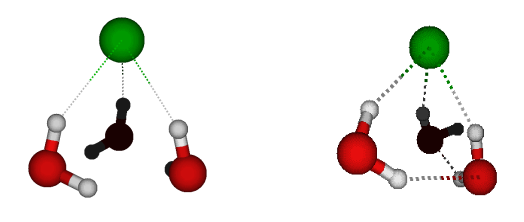
\includegraphics[scale=0.3]{conf_combine.png}
  \caption{These are geometry optimized chloride water clusters
    from AIMD simulations using TPSS-D3/def2-TZVP. Conformation 1
    is on the left and conformation 2 is on the right which will
    be referenced on the tables.}
  \label{fig:conf}
\end{figure}

From the AIMD trajectory of approximately 2 ps, 5 chloride
water clusters were selected within 4.40 kcal/mol difference.
Additional geometry refinement to the 5 structures yielded only
2 unique conformations as seen in Fig \ref{fig:conf}. The
difference between the structures is the hydrogen network
prevalent within the water cluster. However, it appears that
the more stable conformation is the hydrogen bonded to the
chloride ion. This can be seen by the conformation 1 having
a higher free energy and minimum energy, which include
zero vibrational energy, than conformation 2 indicated in
Tables \ref{tab:energies} and \ref{tab:energies2}.

\begin{table}[htbp]
\caption{These are reported chemical potential and free energy
  of the chloride water cluster conformations.}
\begin{tabular}{R|RRR}
  \text{Conformation} & \text{Temperature(K)}&
  \text{Chemical Potential(kJ/mol)}&
  \text{Free Energy(kJ/mol)}\\
  \hline
  1&0.00&-&197.50 \\
   &298.15&112.07& \\
  2&0.00&-&193.65 \\
   &298.15&103.99& \\
\end{tabular}
\label{tab:energies}
\end{table}

\begin{table}[htbp]
\caption{These are repoted energy, enthalpy, and entropy
  of the cholride water cluster conformations.}
\begin{tabular}{R|RRRR}
  \text{Conformation} & \text{Temperature(K)}&
  \text{Energy(kJ/mol)}&
  \text{Enthalpy(kJ/mol)} & \text{Entropy(kJ/mol)} \\
  \hline
  1&0.00&197.50&197.50&- \\
   &298.15&219.43&221.91&0.36841 \\
  2&0.00&193.65&193.65&- \\
   &298.15&217.58&220.06&0.38929 \\
\end{tabular}
\label{tab:energies2}
\end{table}

The detachment energies of comformation 1 and 2 are 115.0 kcal/mol and
114.9 kcal/mol, respectively. In comparison to the PES experiments,
the reported detachment energy is approximately 126.8 kcal/mol which
is approximately 11 kcal/mol difference from the computed detachement
energies of the structures\cite{doi:10.1063/1.467965}. In addition, from Fig \ref{fig:conf_IR}
the computed vibrational spectrum of comformation 2 appears to match
more closely to experimental IR spectra than conformation 1. The computed
band positions of conformation 2 are 3355, 3584, and 3679 wavenumbers
which correspond fairly close to the experimental IR spectra of
3310, 3354, 3391, 3585, and 3600 wavenumbers\cite{doi:10.1063/1.478616}.
Only two additional bands were experimental observed that were not
predicted by the computation.

\begin{figure}[H]
  \centering
  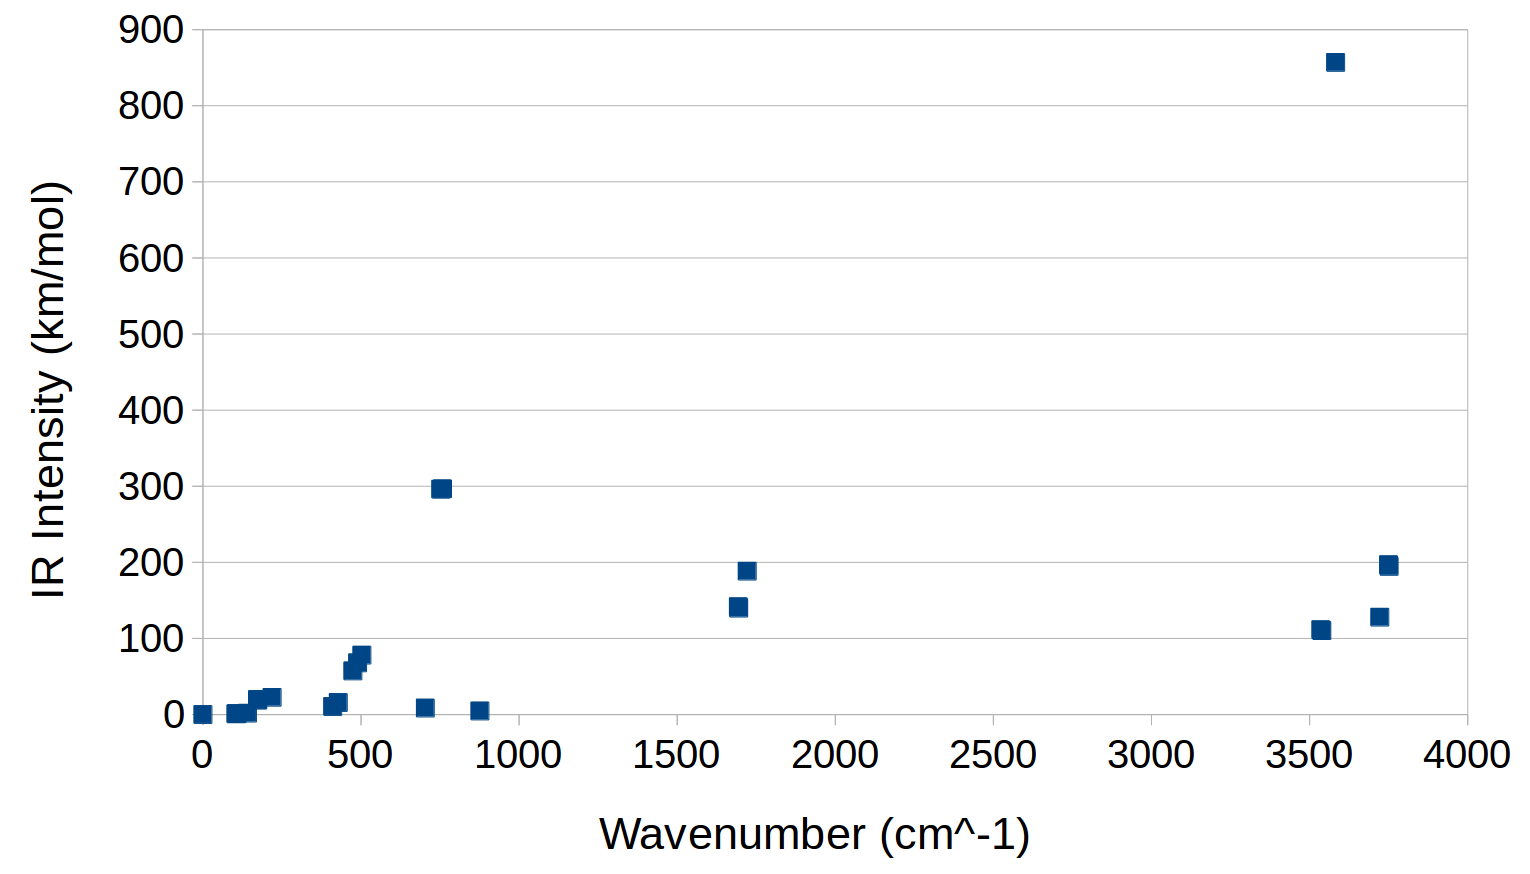
\includegraphics[width=0.35\textwidth]{conf_1IR.png}
  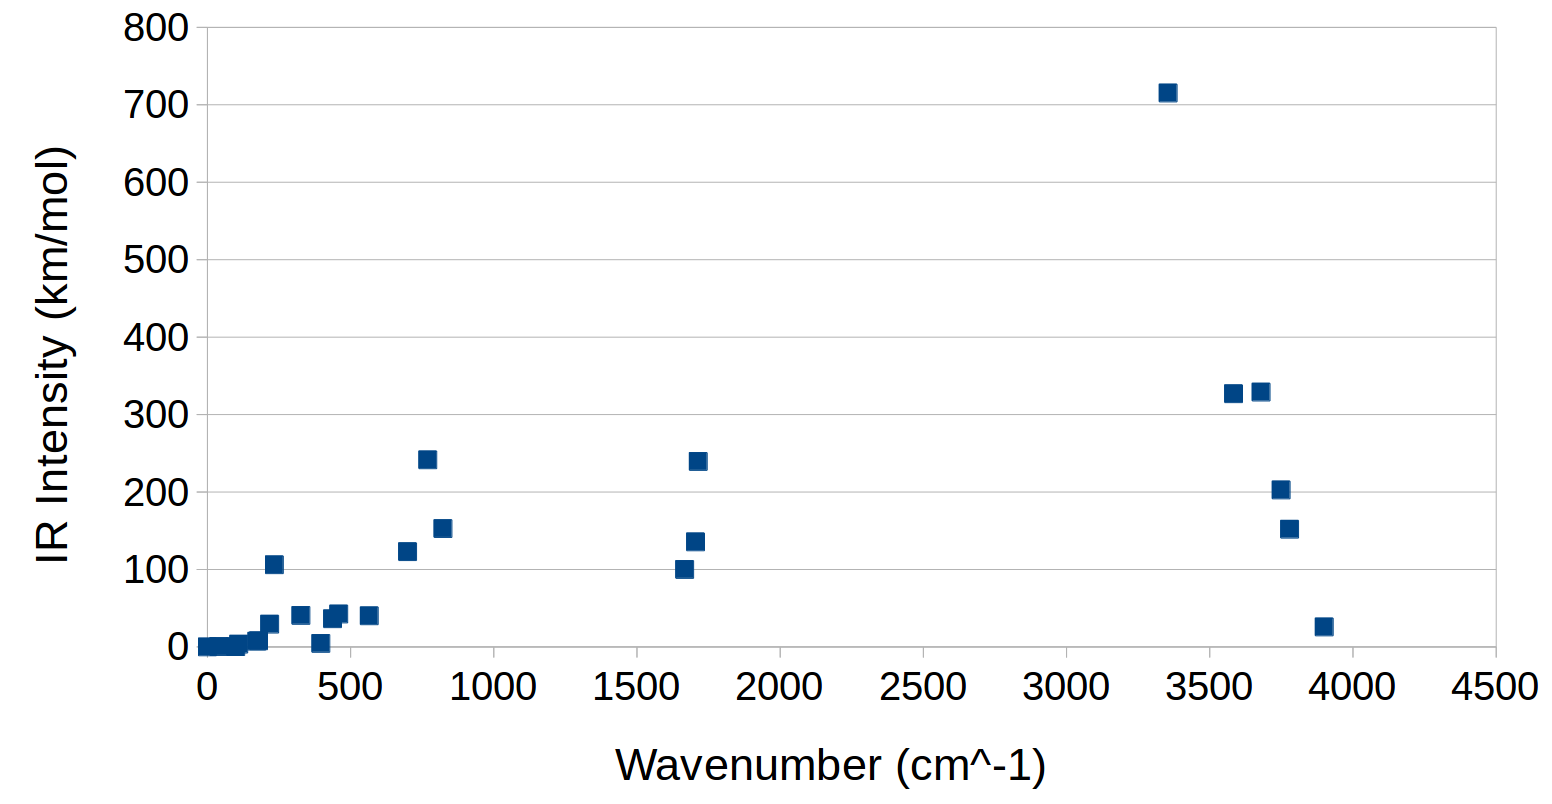
\includegraphics[width=0.35\textwidth]{conf_2IR.png}
  \caption{The computed IR spectrum of conformation 1 (Left) and
    conformation 2 (Right).}
  \label{fig:conf_IR}
\end{figure}

\section{Conclusions}

In conclusion, two structures were found to be local minimas of the chloride
water clusters and only one structure appears to fairly match the experimentally
determined IR spectrum. The only structural difference between the two conformations
is the appearance of the hydrogen network within the water cluster. This suggested
a competition between hydrogen bond networking and the solvation of the
chloride ion. Meanwhile, the overall energy of conformation 1 is lower than
conformation 2 suggesting that conformation 1 is potentially the global
minima. However, this contrasts the experimental results which are in better
agreement with conformation 2. Further sampling may be needed to investigate
the potential energy surface of the chloride water clusters.

\printbibliography

\end{document}
